\chapter{Interpretable Classification Rules}

\section{Experimental Comparison between Incremental vs.\ Non-incremental  Encoding}
We compare the performance of two encoding techniques, na\"ive non-incremental encoding and efficient incremental encoding in {\imli}, for learning interpretable CNF classification rules in datasets of various sizes. We demonstrate the scalability results using a cactus plot in Figure~\ref{fig:interpretability_imli_additional_fig:scalability_non_incremental_vs_incremental}. Each point $ (x, y) $ represents the ability to solve $ x $ classification instances within $ y $ seconds. We test both incremental and non-incremental encoding using $ 360 $ instances for each dataset with varying hyper-parameters. As the dataset size increases, the non-incremental encoding times out, failing to solve all $ 360 $ instances within $ 1000 $ seconds in the Credit and Adult datasets. In contrast, the incremental encoding in {\imli} demonstrates higher scalability, solving all $ 360 $ instances in less than $ 10 $ seconds in the Titanic dataset, and efficiently solving all $ 360 $ instances within the timeout in the Credit and Adult datasets. Hence, the incremental encoding is superior in terms of scalability compared to the non-incremental encoding.

In Figure~\ref{fig:interpretability_imli_additional_fig:all_preformances_non_incremental_vs_incremental}, 

\begin{figure}
	\centering
	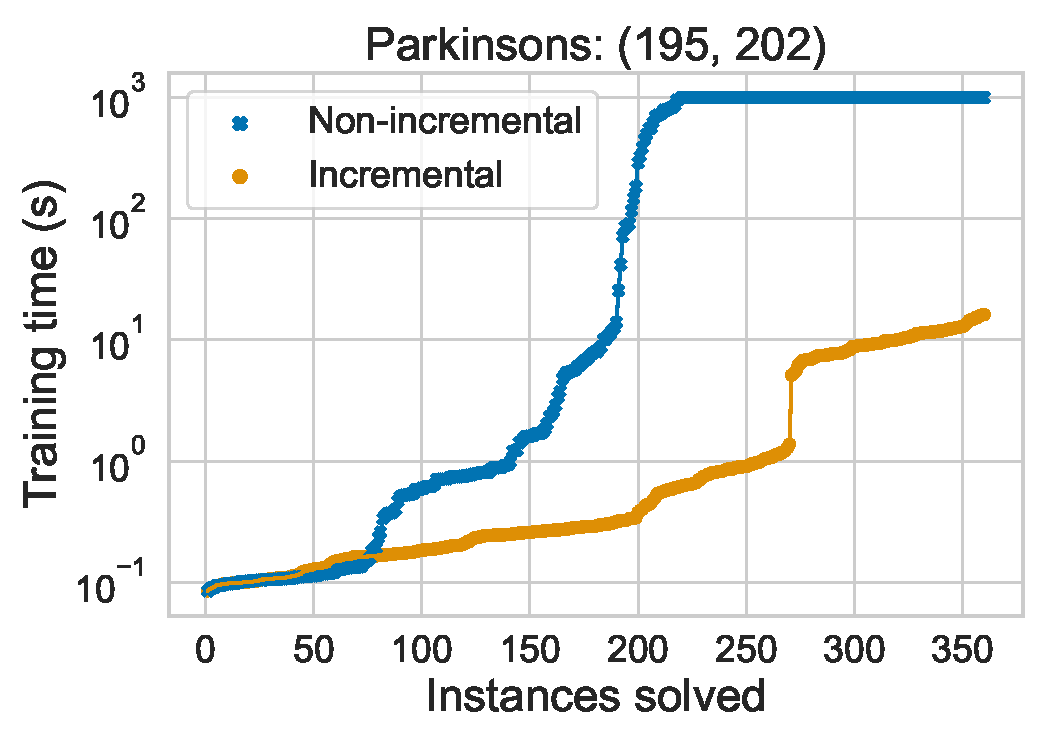
\includegraphics[scale=0.27]{figures/interpretability/imli/thesis_exp/thesis_exp_Parkinsons_cactus_train_val_fit_time}	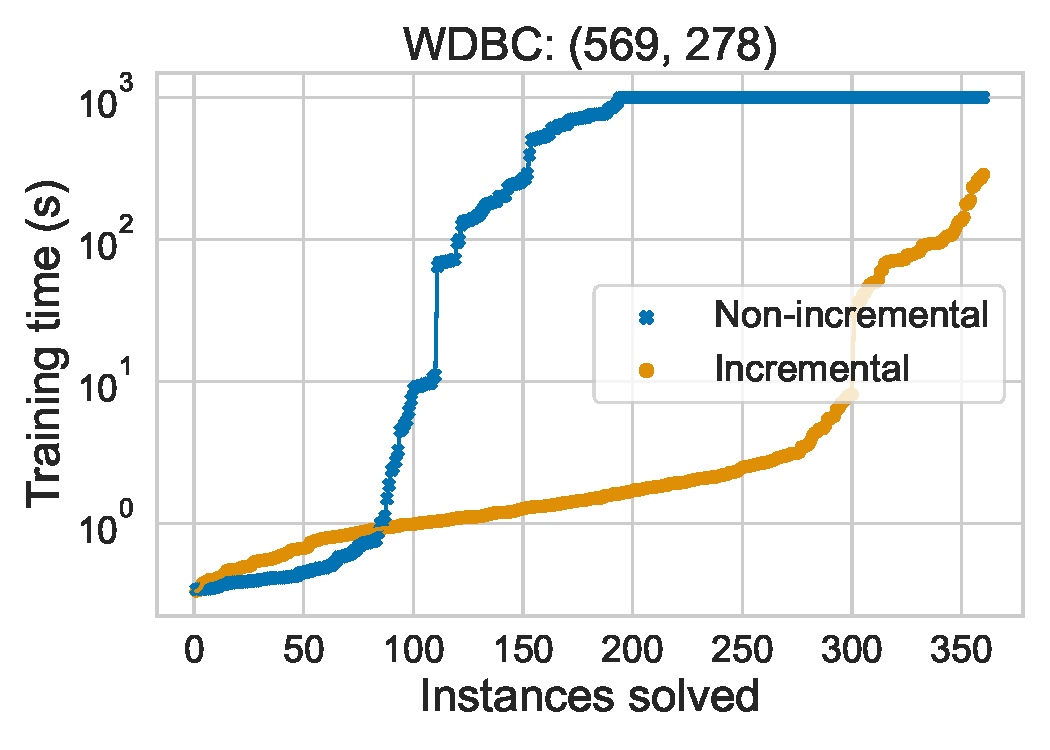
\includegraphics[scale=0.27]{figures/interpretability/imli/thesis_exp/thesis_exp_WDBC_cactus_train_val_fit_time}	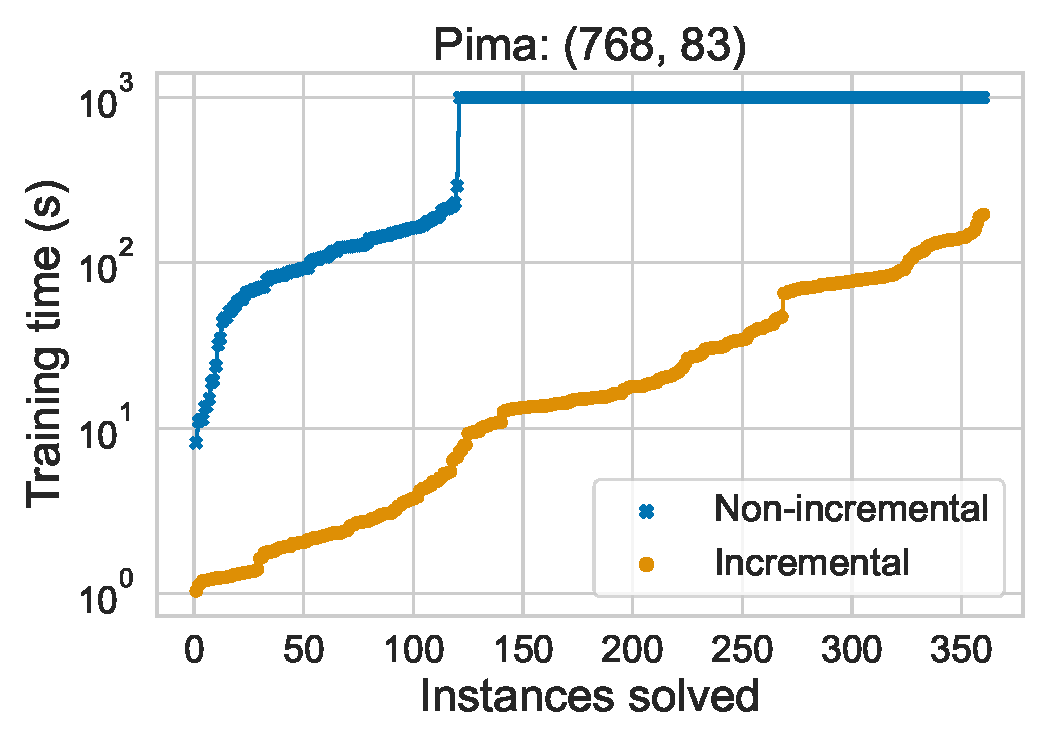
\includegraphics[scale=0.27]{figures/interpretability/imli/thesis_exp/thesis_exp_Pima_cactus_train_val_fit_time}	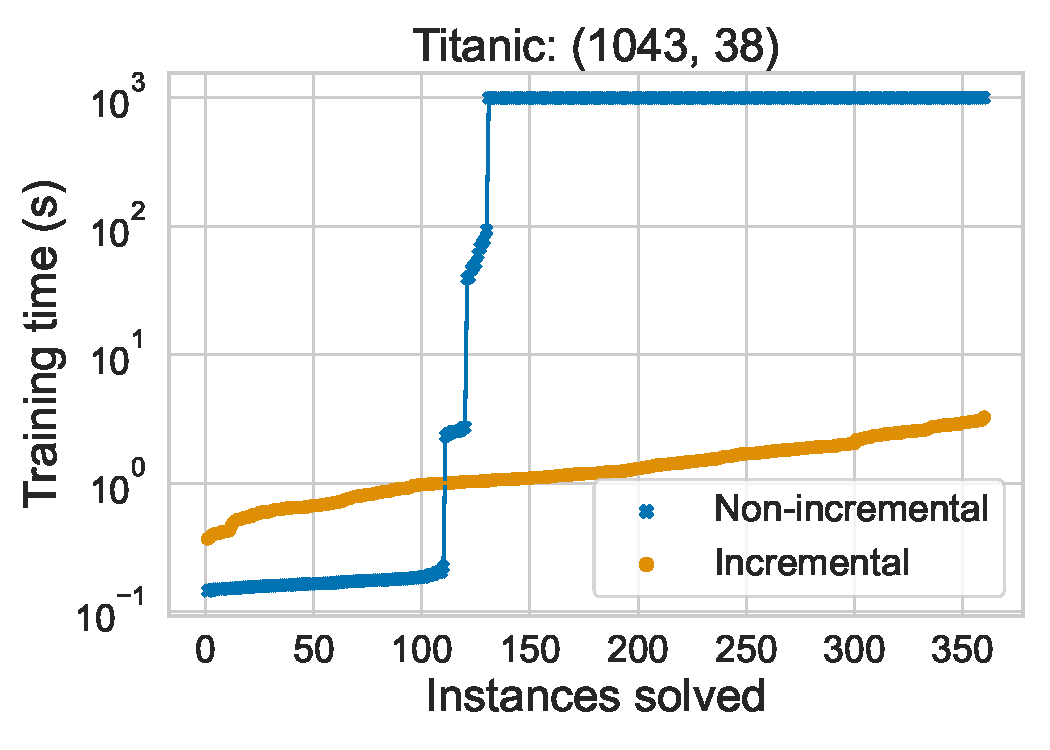
\includegraphics[scale=0.27]{figures/interpretability/imli/thesis_exp/thesis_exp_Titanic_cactus_train_val_fit_time}	\includegraphics[scale=0.27]{figures/interpretability/imli/thesis_exp/thesis_exp_Magic_cactus_train_val_fit_time}	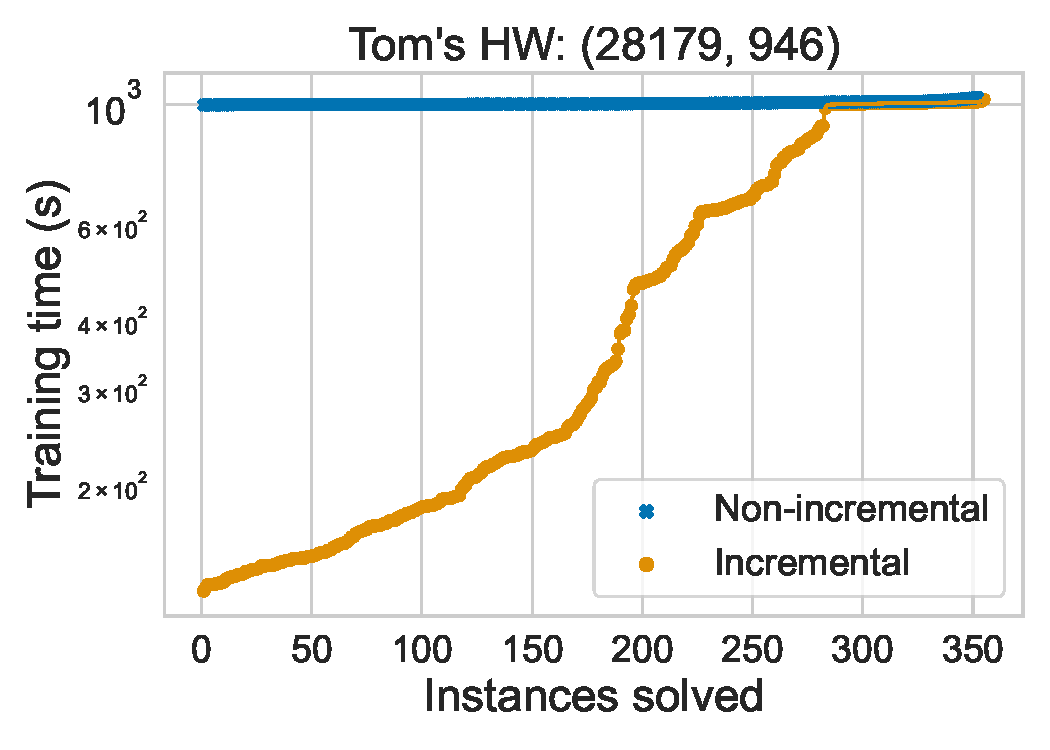
\includegraphics[scale=0.27]{figures/interpretability/imli/thesis_exp/thesis_exp_Tom's_HW_cactus_train_val_fit_time}		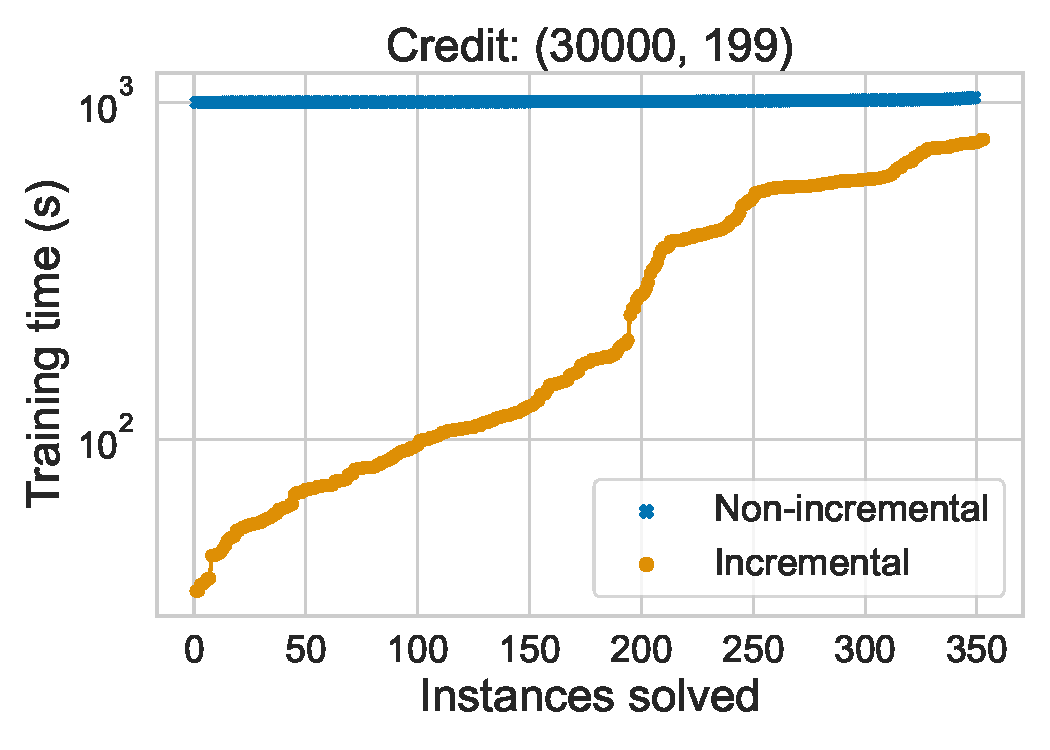
\includegraphics[scale=0.27]{figures/interpretability/imli/thesis_exp/thesis_exp_Credit_cactus_train_val_fit_time}	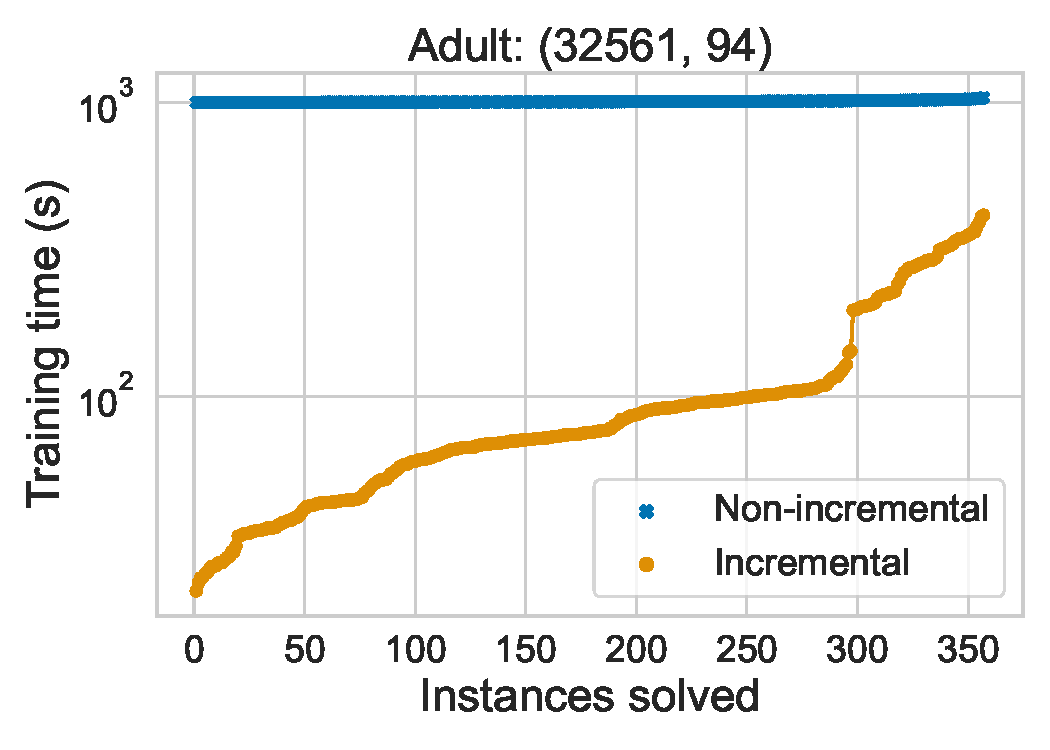
\includegraphics[scale=0.27]{figures/interpretability/imli/thesis_exp/thesis_exp_Adult_cactus_train_val_fit_time}
	\caption[Scalability: incremental vs.\ non-incremental encoding]{Detailed scalability results of incremental vs.\ non-incremental encoding in {\imli}, presented as a cactus plot. As datasets become large, the non-incremental encoding suffers from poor scalability by witnessing time-outs more frequently than the incremental encoding {\imli}.}
	\label{fig:interpretability_imli_additional_fig:scalability_non_incremental_vs_incremental}
\end{figure}


\begin{figure}
	\centering
	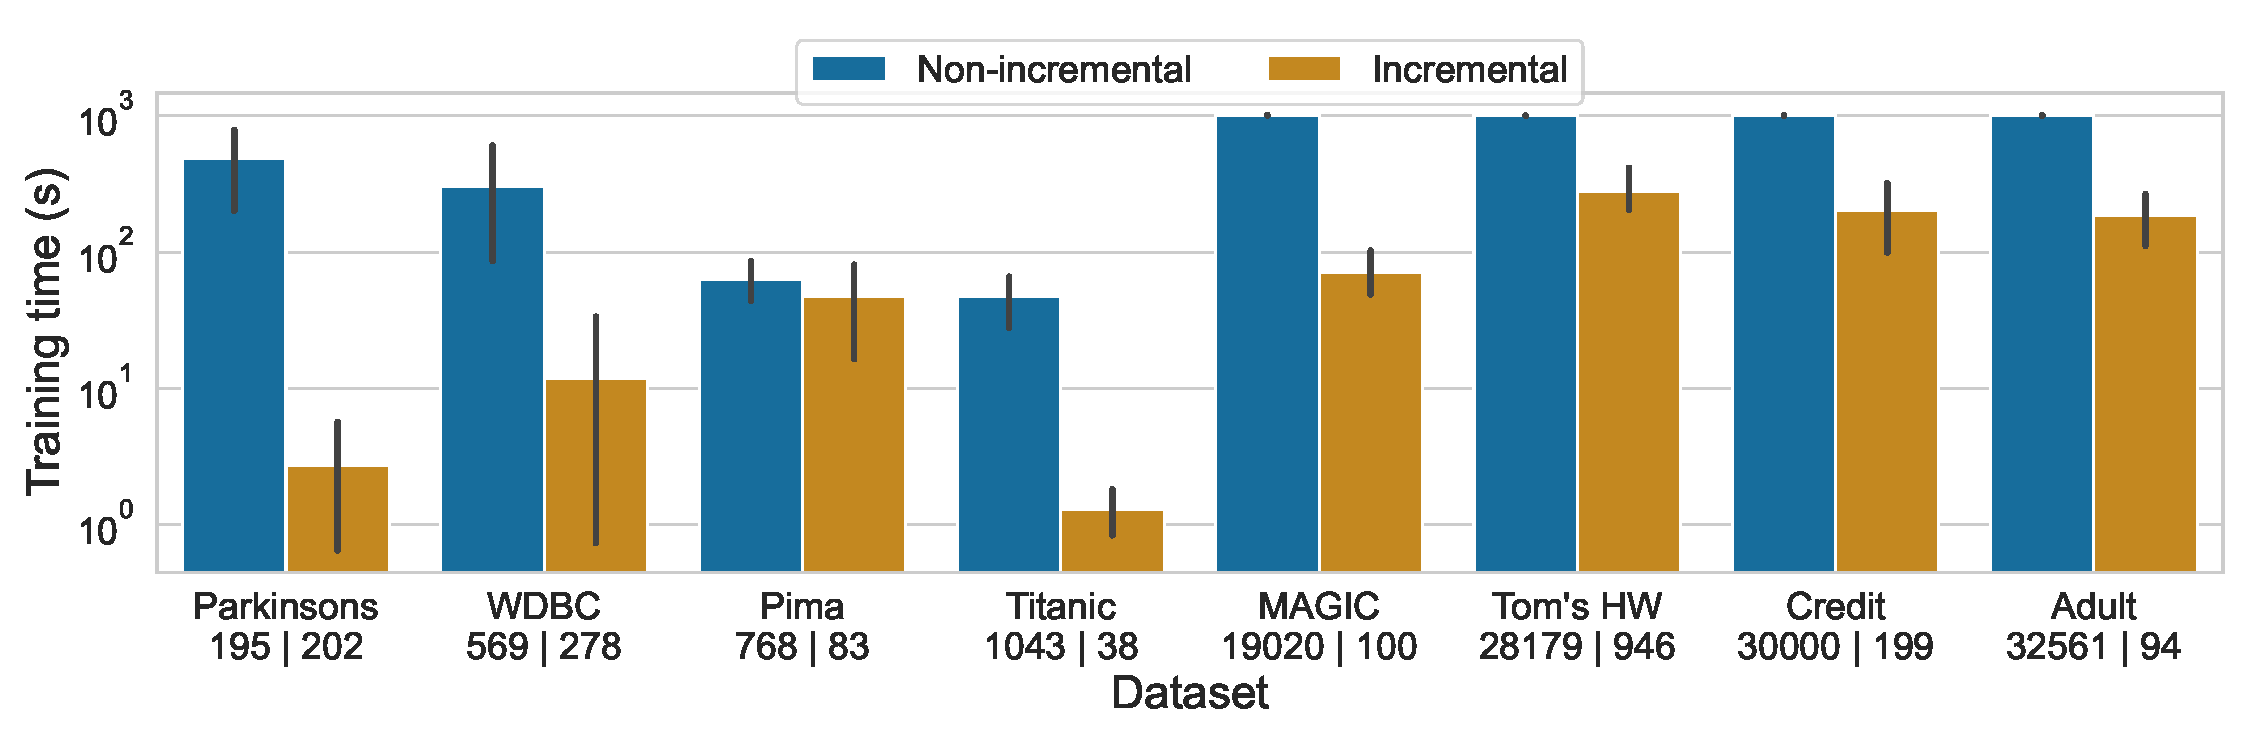
\includegraphics[scale=0.38]{figures/interpretability/imli/thesis_exp/thesis_exp_cactus_train_val_fit_time}
	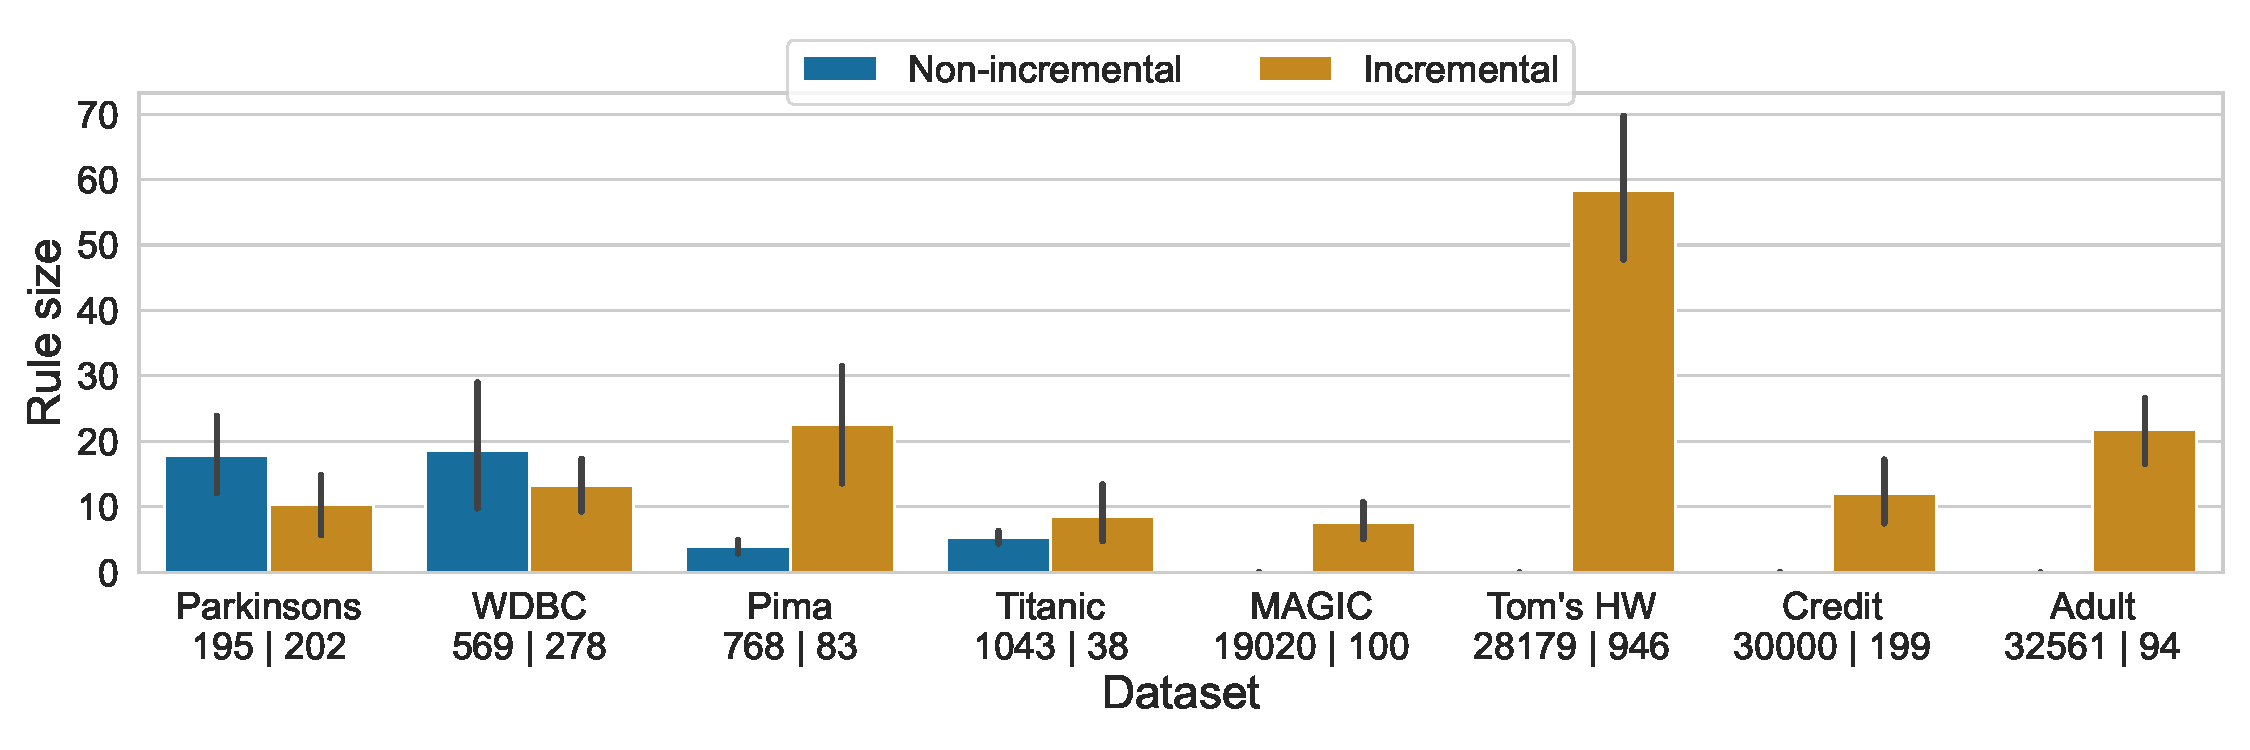
\includegraphics[scale=0.38]{figures/interpretability/imli/thesis_exp/thesis_exp_cactus_predicate_count}
	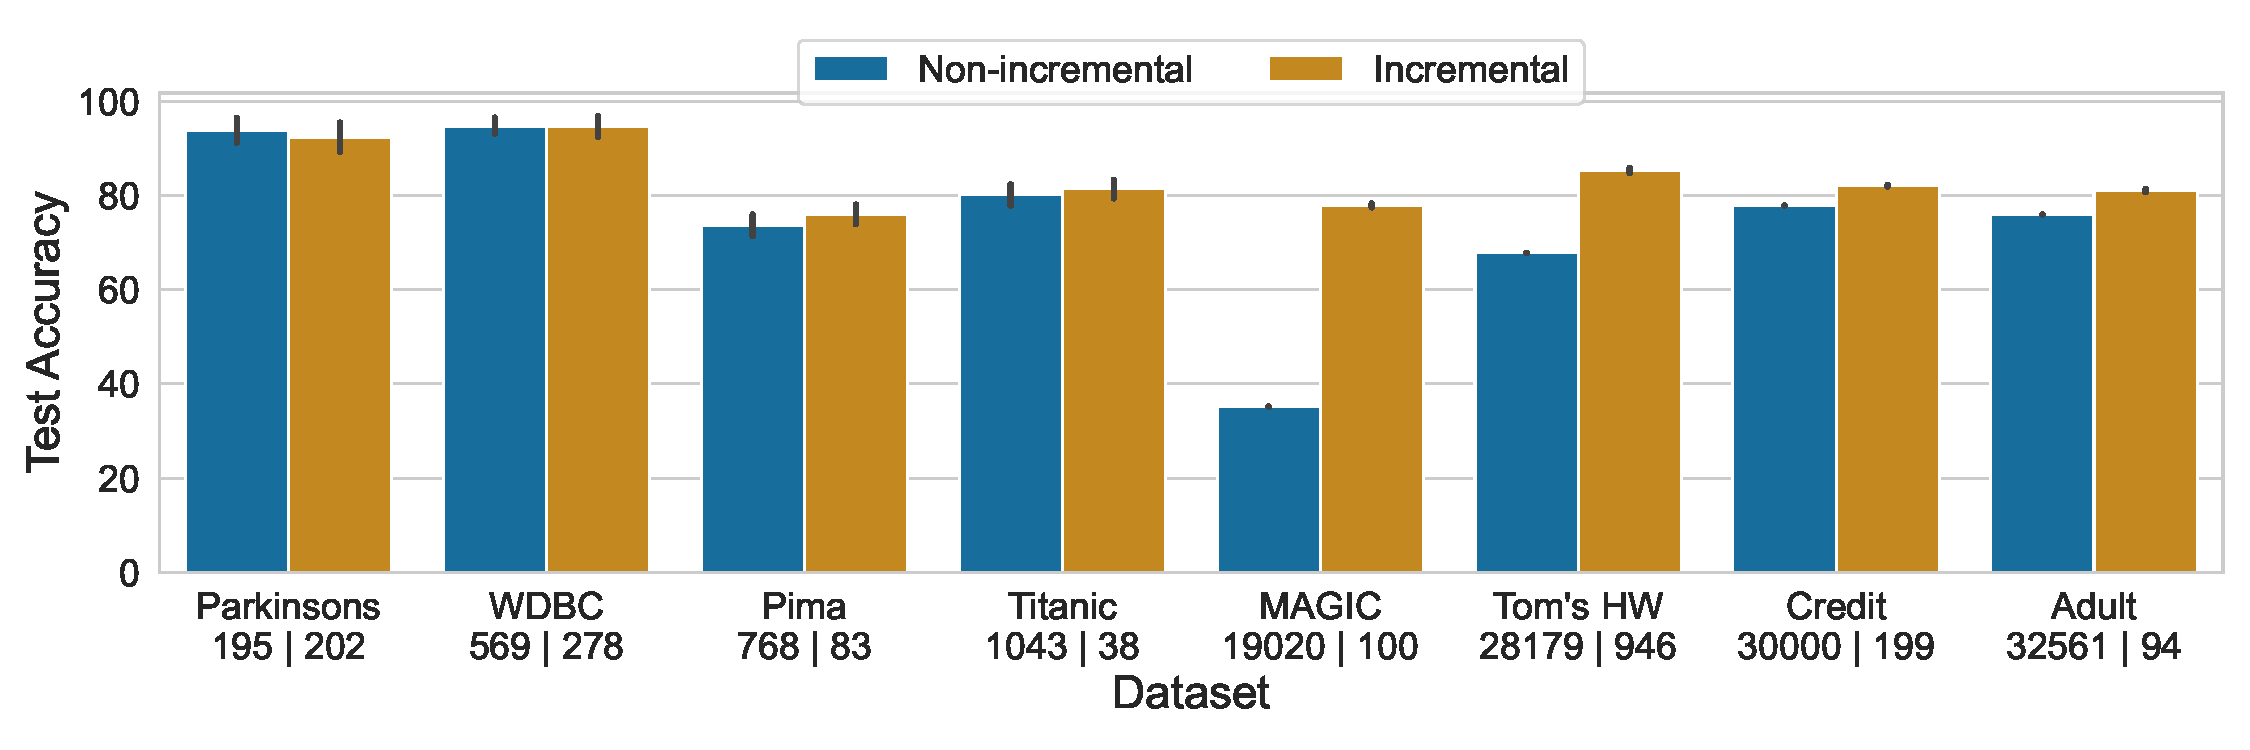
\includegraphics[scale=0.38]{figures/interpretability/imli/thesis_exp/thesis_exp_cactus_test_accuracy}
	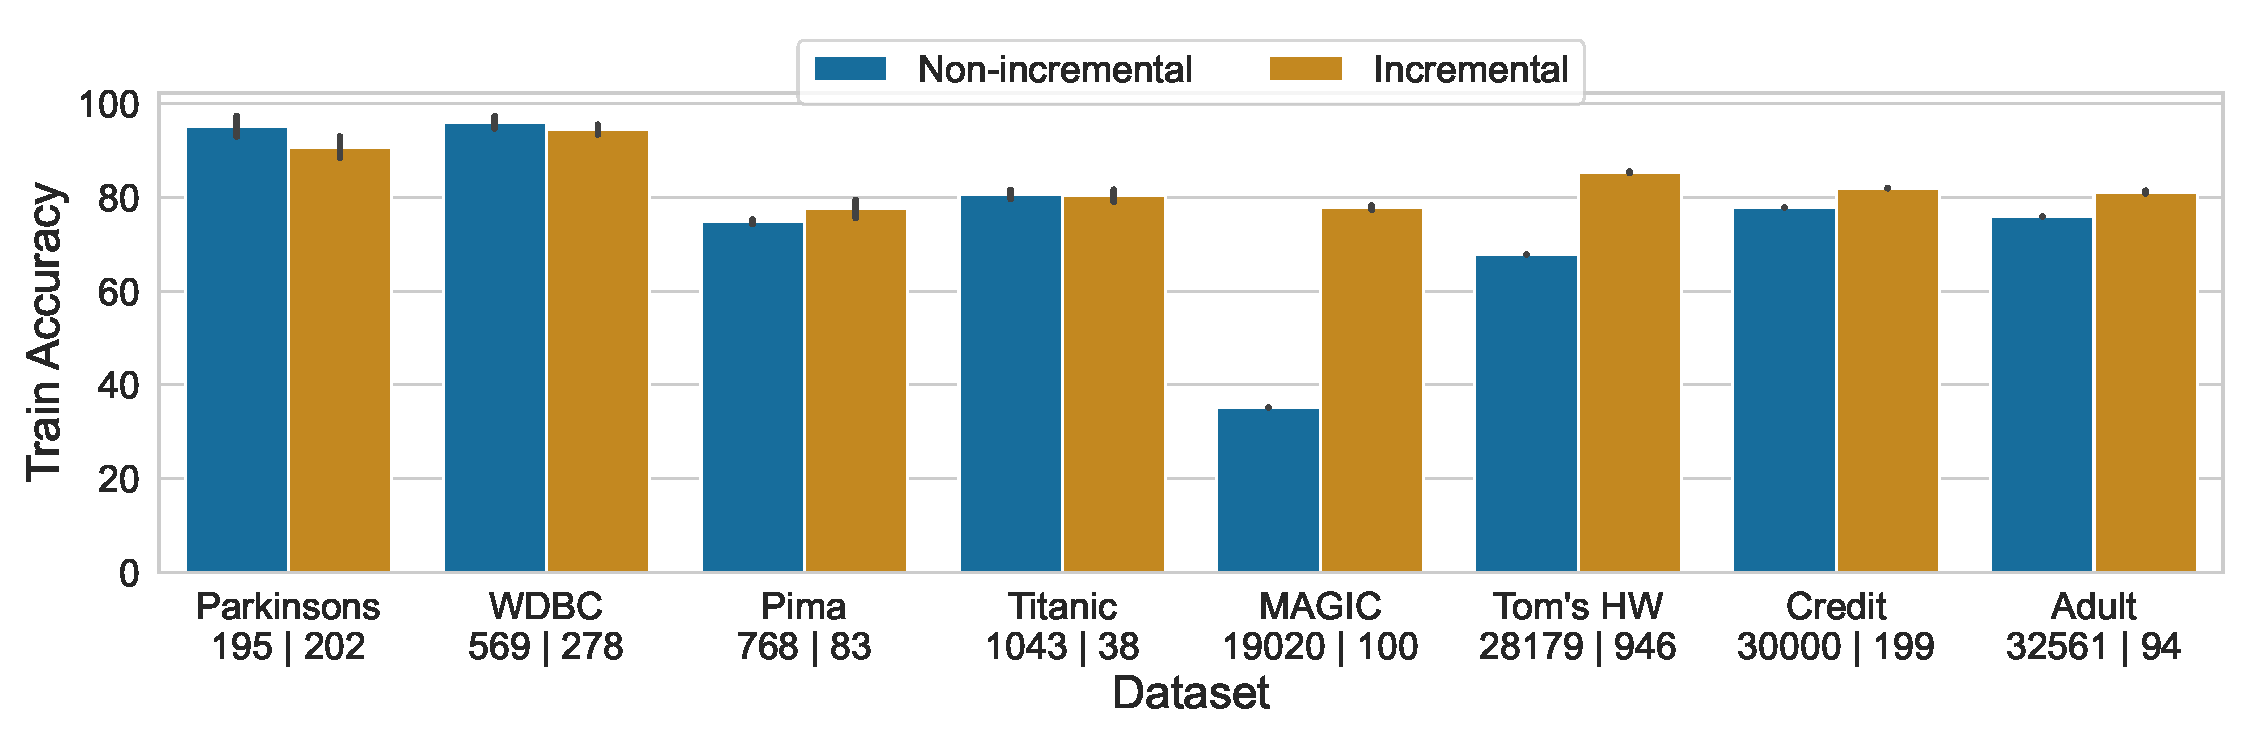
\includegraphics[scale=0.38]{figures/interpretability/imli/thesis_exp/thesis_exp_cactus_train_val_accuracy}
	
	\caption[Performance comparison between non-incremental vs.\ incremental encoding]{Comparison of training time, rule-size, and test and train accuracy between non-incremental vs.\ incremental encoding in {\imli}. In $ X $-axis, the dimension of the dataset (\#samples $ \mid $  \#features) is shown below dataset name. In large datasets, non-incremental encoding often times out and learns zero-size classification rules yielding less test and train accuracy than the incremental encoding.}
	\label{fig:interpretability_imli_additional_fig:all_preformances_non_incremental_vs_incremental}
\end{figure}




\section{Representative Interpretable Classifiers}
In the following, we present representative CNF classifiers learned in different datasets. In each dataset, if an input satisfies the CNF formula, it is predicted class $ 1 $ and vice-versa.

\noindent \textbf{ Parkinsons: }\\

\noindent 0.3 $\le$ Average vocal fundamental frequency $<$ 0.4 \textbf{OR} 0.5 $\le$ Average vocal fundamental frequency $<$ 0.6 \textbf{OR} 0.1 $\le$ Maximum vocal fundamental frequency $<$ 0.2 \textbf{OR} 0.5 $\le$ Minimum vocal fundamental frequency $<$ 0.6 \textbf{OR} 0.1 $\le$ Shimmer:APQ5 $<$ 0.2 \textbf{OR} 0.5 $\le$ DFA $<$ 0.6 \textbf{OR} 0.3 $\le$ spread1 $<$ 0.4 \textbf{OR} 0.8 $\le$ spread2 $<$ 0.9 \textbf{OR} 0.3 $\le$ PPE $<$ 0.4 \textbf{OR}  \textbf{NOT} -$\infty$ $\le$ MDVP:APQ $<$ 0.1 \blue{\textbf{AND}}\\\\ \textbf{NOT} 0.8 $\le$ Average vocal fundamental frequency $<$ 0.9 \\

\noindent \textbf{ WDBC: }\\

\noindent 0.4 $\le$ perimeter $<$ 0.5 \textbf{OR} 0.8 $\le$ symmetry $<$ 0.9 \textbf{OR} 0.5 $\le$ largest concave points $<$ 0.6 \textbf{OR} 0.6 $\le$ largest concave points $<$ 0.7 \textbf{OR} 0.7 $\le$ largest concave points $<$ 0.8 \textbf{OR} 0.6 $\le$ largest symmetry $<$ 0.7 \textbf{OR}  \textbf{NOT} -$\infty$ $\le$ area SE $<$ 0.1 \blue{\textbf{AND}}\\\\0.4 $\le$ texture $<$ 0.5 \textbf{OR} 0.5 $\le$ texture $<$ 0.6 \textbf{OR} 0.5 $\le$ perimeter $<$ 0.6 \textbf{OR} 0.5 $\le$ smoothness $<$ 0.6 \textbf{OR} 0.4 $\le$ concave points $<$ 0.5 \textbf{OR} 0.5 $\le$ concave points $<$ 0.6 \textbf{OR} 0.2 $\le$ largest concavity $<$ 0.3 \textbf{OR} 0.6 $\le$ largest concave points $<$ 0.7 \textbf{OR} 0.7 $\le$ largest concave points $<$ 0.8 \textbf{OR} 0.4 $\le$ largest symmetry $<$ 0.5 \textbf{OR} 0.6 $\le$ largest symmetry $<$ 0.7 \\

\noindent \textbf{ Pima: }\\

\noindent x1 = 11 \textbf{OR} x1 = 14 \textbf{OR} x1 = 15 \textbf{OR} 0.7 $\le$ x2 $<$ 0.8 \textbf{OR} 0.8 $\le$ x2 $<$ 0.9 \textbf{OR} 0.9 $\le$ x2 $<$ $\infty$ \textbf{OR} 0.9 $\le$ x3 $<$ $\infty$ \textbf{OR} 0.4 $\le$ x5 $<$ 0.5 \textbf{OR} 0.7 $\le$ x5 $<$ 0.8 \textbf{OR} 0.7 $\le$ x6 $<$ 0.8 \textbf{OR} 0.4 $\le$ x7 $<$ 0.5 \textbf{OR} 0.5 $\le$ x7 $<$ 0.6 \textbf{OR} 0.9 $\le$ x7 $<$ $\infty$ \blue{\textbf{AND}}\\\\x1 = 7 \textbf{OR} x1 = 8 \textbf{OR} 0.6 $\le$ x2 $<$ 0.7 \textbf{OR} 0.8 $\le$ x2 $<$ 0.9 \textbf{OR} 0.9 $\le$ x2 $<$ $\infty$ \textbf{OR} -$\infty$ $\le$ x3 $<$ 0.1 \textbf{OR} 0.7 $\le$ x3 $<$ 0.8 \textbf{OR} 0.9 $\le$ x3 $<$ $\infty$ \textbf{OR} 0.2 $\le$ x5 $<$ 0.3 \textbf{OR} 0.7 $\le$ x6 $<$ 0.8 \textbf{OR} 0.1 $\le$ x7 $<$ 0.2 \textbf{OR} 0.3 $\le$ x7 $<$ 0.4 \textbf{OR} 0.4 $\le$ x8 $<$ 0.5 \textbf{OR} 0.8 $\le$ x8 $<$ 0.9 \blue{\textbf{AND}}\\\\x1 = 2 \textbf{OR} x1 = 6 \textbf{OR} x1 = 7 \textbf{OR} x1 = 9 \textbf{OR} -$\infty$ $\le$ x3 $<$ 0.1 \textbf{OR} 0.8 $\le$ x3 $<$ 0.9 \textbf{OR} 0.1 $\le$ x5 $<$ 0.2 \textbf{OR} 0.2 $\le$ x5 $<$ 0.3 \textbf{OR} 0.7 $\le$ x5 $<$ 0.8 \textbf{OR} 0.5 $\le$ x6 $<$ 0.6 \textbf{OR} 0.6 $\le$ x6 $<$ 0.7 \textbf{OR} 0.4 $\le$ x7 $<$ 0.5 \textbf{OR} 0.9 $\le$ x7 $<$ $\infty$ \textbf{OR} 0.1 $\le$ x8 $<$ 0.2 \textbf{OR} 0.3 $\le$ x8 $<$ 0.4 \textbf{OR} 0.6 $\le$ x8 $<$ 0.7 \textbf{OR} 0.8 $\le$ x8 $<$ 0.9 \blue{\textbf{AND}}\\\\x1 = 8 \textbf{OR} 0.5 $\le$ x2 $<$ 0.6 \textbf{OR} 0.8 $\le$ x2 $<$ 0.9 \textbf{OR} 0.9 $\le$ x2 $<$ $\infty$ \textbf{OR} 0.7 $\le$ x3 $<$ 0.8 \textbf{OR} -$\infty$ $\le$ x4 $<$ 0.1 \textbf{OR} 0.1 $\le$ x5 $<$ 0.2 \textbf{OR} 0.3 $\le$ x5 $<$ 0.4 \textbf{OR} 0.5 $\le$ x7 $<$ 0.6 \textbf{OR} 0.1 $\le$ x8 $<$ 0.2 \textbf{OR} 0.4 $\le$ x8 $<$ 0.5 \textbf{OR} 0.8 $\le$ x8 $<$ 0.9 \\

\noindent \textbf{ Titanic: }\\

\noindent -$\infty$ $\le$ age $<$ 0.1 \textbf{OR} 0.9 $\le$ age $<$ $\infty$ \textbf{OR} 0.9 $\le$ fare $<$ $\infty$ \textbf{OR}  \textbf{NOT} sex \blue{\textbf{AND}}\\\\passenger-class = 2 \textbf{OR} 0.4 $\le$ age $<$ 0.5 \textbf{OR} 0.6 $\le$ age $<$ 0.7 \textbf{OR} siblings-or-spouces-aboard = 0 \textbf{OR} 0.1 $\le$ fare $<$ 0.2 \textbf{OR} 0.5 $\le$ fare $<$ 0.6 \textbf{OR} embarked = C \blue{\textbf{AND}}\\\\-$\infty$ $\le$ age $<$ 0.1 \textbf{OR} 0.1 $\le$ age $<$ 0.2 \textbf{OR} 0.7 $\le$ age $<$ 0.8 \textbf{OR} siblings-or-spouces-aboard = 1 \textbf{OR} parents-or-childred-aboard = 1 \textbf{OR} embarked = C \textbf{OR}  \textbf{NOT} passenger-class = 3 \blue{\textbf{AND}}\\\\-$\infty$ $\le$ age $<$ 0.1 \textbf{OR} 0.2 $\le$ age $<$ 0.3 \textbf{OR} 0.3 $\le$ age $<$ 0.4 \textbf{OR} parents-or-childred-aboard = 0 \textbf{OR}  \textbf{NOT} passenger-class = 3 \textbf{OR}  \textbf{NOT} siblings-or-spouces-aboard = 0 \blue{\textbf{AND}}\\\\ \textbf{NOT} passenger-class = 2 \textbf{OR}  \textbf{NOT} 0.7 $\le$ age $<$ 0.8 \\

\noindent \textbf{ MAGIC: }\\

\noindent -$\infty$ $\le$ length $<$ 0.1 \textbf{OR} -$\infty$ $\le$ size $<$ 0.1 \textbf{OR} 0.8 $\le$ conc $<$ 0.9 \textbf{OR} -$\infty$ $\le$ alpha $<$ 0.1 \textbf{OR} 0.1 $\le$ alpha $<$ 0.2 \textbf{OR} 0.2 $\le$ dist $<$ 0.3 \\

\noindent \textbf{ Tom's HW: }\\

\noindent 0.4 $\le$ x10 $<$ 0.5 \textbf{OR} 0.1 $\le$ x11 $<$ 0.2 \textbf{OR} 0.4 $\le$ x11 $<$ 0.5 \textbf{OR} 0.4 $\le$ x12 $<$ 0.5 \textbf{OR} 0.3 $\le$ x13 $<$ 0.4 \textbf{OR} 0.6 $\le$ x13 $<$ 0.7 \textbf{OR} 0.3 $\le$ x15 $<$ 0.4 \textbf{OR} 0.6 $\le$ x15 $<$ 0.7 \textbf{OR} 0.4 $\le$ x16 $<$ 0.5 \textbf{OR} 0.1 $\le$ x57 $<$ 0.2 \textbf{OR} 0.5 $\le$ x59 $<$ 0.6 \textbf{OR} 0.3 $\le$ x60 $<$ 0.4 \textbf{OR} 0.2 $\le$ x62 $<$ 0.3 \textbf{OR} 0.2 $\le$ x73 $<$ 0.3 \textbf{OR} 0.1 $\le$ x74 $<$ 0.2 \textbf{OR}  \textbf{NOT} -$\infty$ $\le$ x74 $<$ 0.1 \textbf{OR}  \textbf{NOT} -$\infty$ $\le$ x96 $<$ 0.1 \blue{\textbf{AND}}\\\\0.4 $\le$ x9 $<$ 0.5 \textbf{OR} 0.8 $\le$ x9 $<$ 0.9 \textbf{OR} 0.2 $\le$ x12 $<$ 0.3 \textbf{OR} 0.3 $\le$ x12 $<$ 0.4 \textbf{OR} 0.3 $\le$ x15 $<$ 0.4 \textbf{OR} 0.6 $\le$ x15 $<$ 0.7 \textbf{OR} 0.1 $\le$ x60 $<$ 0.2 \textbf{OR} 0.1 $\le$ x61 $<$ 0.2 \textbf{OR} 0.6 $\le$ x78 $<$ 0.7 \textbf{OR}  \textbf{NOT} -$\infty$ $\le$ x11 $<$ 0.1 \textbf{OR}  \textbf{NOT} -$\infty$ $\le$ x13 $<$ 0.1 \textbf{OR}  \textbf{NOT} -$\infty$ $\le$ x46 $<$ 0.1 \textbf{OR}  \textbf{NOT} -$\infty$ $\le$ x64 $<$ 0.1 \textbf{OR}  \textbf{NOT} -$\infty$ $\le$ x72 $<$ 0.1 \textbf{OR}  \textbf{NOT} -$\infty$ $\le$ x77 $<$ 0.1 \blue{\textbf{AND}}\\\\-$\infty$ $\le$ x50 $<$ 0.1 \textbf{OR} 0.1 $\le$ x57 $<$ 0.2 \blue{\textbf{AND}}\\\\-$\infty$ $\le$ x49 $<$ 0.1 \textbf{OR}  \textbf{NOT} -$\infty$ $\le$ x17 $<$ 0.1 \blue{\textbf{AND}}\\\\0.3 $\le$ x14 $<$ 0.4 \textbf{OR} 0.6 $\le$ x74 $<$ 0.7 \textbf{OR} 0.9 $\le$ x79 $<$ $\infty$ \textbf{OR}  \textbf{NOT} -$\infty$ $\le$ x9 $<$ 0.1 \textbf{OR}  \textbf{NOT} -$\infty$ $\le$ x15 $<$ 0.1 \textbf{OR}  \textbf{NOT} -$\infty$ $\le$ x73 $<$ 0.1 \textbf{OR}  \textbf{NOT} -$\infty$ $\le$ x80 $<$ 0.1 \\

\noindent \textbf{ Credit: }\\

\noindent Repayment-status-in-September = 2 \textbf{OR} Repayment-status-in-September = 3 \textbf{OR} Repayment-status-in-August = 3 \textbf{OR} Repayment-status-in-May = 3 \textbf{OR} Repayment-status-in-May = 5 \textbf{OR} Repayment-status-in-April = 3 \blue{\textbf{AND}}\\\\0.4 $\le$ Age $<$ 0.5 \textbf{OR} Repayment-status-in-September = 1 \textbf{OR} Repayment-status-in-August = 0 \textbf{OR} Repayment-status-in-July = 2 \textbf{OR} Repayment-status-in-May = 2 \textbf{OR} Repayment-status-in-April = 7 \textbf{OR} 0.3 $\le$ Amount-of-bill-statement-in-April $<$ 0.4 \textbf{OR}  \textbf{NOT} Repayment-status-in-May = -1 \textbf{OR}  \textbf{NOT} -$\infty$ $\le$ Amount-of-bill-statement-in-May $<$ 0.1 \blue{\textbf{AND}}\\\\Gender \textbf{OR} -$\infty$ $\le$ Age $<$ 0.1 \textbf{OR} 0.3 $\le$ Age $<$ 0.4 \textbf{OR} Repayment-status-in-September = 1 \textbf{OR} 0.1 $\le$ Amount-of-bill-statement-in-August $<$ 0.2 \textbf{OR}  \textbf{NOT} Education = 3 \textbf{OR}  \textbf{NOT} 0.2 $\le$ Amount-of-bill-statement-in-September $<$ 0.3 \\

\noindent \textbf{ Adult: }\\

\noindent education =  Doctorate \textbf{OR} education =  Prof-school \textbf{OR} 0.1 $\le$ capital-gain $<$ 0.2 \textbf{OR} 0.2 $\le$ capital-gain $<$ 0.3 \textbf{OR} 0.9 $\le$ capital-gain $<$ $\infty$ \textbf{OR} 0.4 $\le$ capital-loss $<$ 0.5 \textbf{OR} 0.5 $\le$ capital-loss $<$ 0.6 \blue{\textbf{AND}}\\\\relationship =  Husband \textbf{OR} relationship =  Wife \textbf{OR} 0.5 $\le$ capital-loss $<$ 0.6 \textbf{OR} 0.6 $\le$ capital-loss $<$ 0.7 \textbf{OR} 0.8 $\le$ capital-loss $<$ 0.9 \textbf{OR}  \textbf{NOT} -$\infty$ $\le$ capital-gain $<$ 0.1 \blue{\textbf{AND}}\\\\0.1 $\le$ age $<$ 0.2 \textbf{OR} 0.7 $\le$ age $<$ 0.8 \textbf{OR} workclass =  State-gov \textbf{OR} education =  Bachelors \textbf{OR} marital-status =  Separated \textbf{OR} occupation =  Exec-managerial \textbf{OR} occupation =  Farming-fishing \textbf{OR} occupation =  Prof-specialty \textbf{OR} occupation =  Protective-serv \textbf{OR} occupation =  Tech-support \textbf{OR} relationship =  Unmarried \textbf{OR} 0.4 $\le$ capital-loss $<$ 0.5 \textbf{OR} 0.6 $\le$ capital-loss $<$ 0.7 \textbf{OR} 0.2 $\le$ hours-per-week $<$ 0.3 \textbf{OR} 0.4 $\le$ hours-per-week $<$ 0.5 \textbf{OR} 0.7 $\le$ hours-per-week $<$ 0.8 \textbf{OR} 0.9 $\le$ hours-per-week $<$ $\infty$ \textbf{OR}  \textbf{NOT} -$\infty$ $\le$ capital-gain $<$ 0.1 \\

\noindent \textbf{ Bank Marketing: }\\

\noindent 0.7 $\le$ age $<$ 0.8 \textbf{OR} 0.2 $\le$ duration $<$ 0.3 \textbf{OR} 0.3 $\le$ duration $<$ 0.4 \textbf{OR} 0.4 $\le$ duration $<$ 0.5 \textbf{OR} 0.5 $\le$ duration $<$ 0.6 \textbf{OR} poutcome = success \blue{\textbf{AND}}\\\\housing \textbf{OR} 0.8 $\le$ age $<$ 0.9 \textbf{OR} job = admin. \textbf{OR} job = management \textbf{OR} job = self-employed \textbf{OR} job = services \textbf{OR} job = unemployed \textbf{OR} 0.2 $\le$ duration $<$ 0.3 \textbf{OR} 0.1 $\le$ campaign $<$ 0.2 \textbf{OR} poutcome = success \blue{\textbf{AND}}\\\\job = services \textbf{OR} 0.2 $\le$ balance $<$ 0.3 \textbf{OR} contact = cellular \textbf{OR} 0.1 $\le$ duration $<$ 0.2 \textbf{OR} 0.2 $\le$ duration $<$ 0.3 \textbf{OR} 0.2 $\le$ pdays $<$ 0.3 \textbf{OR} poutcome = unknown \textbf{OR}  \textbf{NOT} -$\infty$ $\le$ balance $<$ 0.1 \textbf{OR}  \textbf{NOT} -$\infty$ $\le$ previous $<$ 0.1 \blue{\textbf{AND}}\\\\0.2 $\le$ age $<$ 0.3 \textbf{OR} 0.3 $\le$ age $<$ 0.4 \textbf{OR} 0.8 $\le$ age $<$ 0.9 \textbf{OR} job = management \textbf{OR} job = student \textbf{OR} job = unemployed \textbf{OR} education = secondary \textbf{OR} 0.1 $\le$ balance $<$ 0.2 \textbf{OR} 0.1 $\le$ duration $<$ 0.2 \textbf{OR} -$\infty$ $\le$ pdays $<$ 0.1 \textbf{OR} 0.2 $\le$ pdays $<$ 0.3 \textbf{OR} poutcome = unknown \\

\noindent \textbf{ Connect-4: }\\

\noindent b2 = 1 \textbf{OR} c2 = 1 \textbf{OR} d2 = 1 \textbf{OR} d4 = 1 \textbf{OR} d5 = 0 \textbf{OR} e2 = 1 \textbf{OR} f3 = 0 \textbf{OR}  \textbf{NOT} d1 = 0 \blue{\textbf{AND}}\\\\b2 = 1 \textbf{OR} b3 = 1 \textbf{OR} b4 = 1 \textbf{OR} d4 = 1 \textbf{OR} f2 = 1 \textbf{OR}  \textbf{NOT} d3 = 0 \textbf{OR}  \textbf{NOT} f3 = 2 \blue{\textbf{AND}}\\\\c1 = 2 \textbf{OR} c2 = 2 \textbf{OR} c3 = 1 \textbf{OR} c3 = 2 \textbf{OR} c4 = 1 \textbf{OR} c6 = 0 \textbf{OR} d2 = 1 \textbf{OR} d4 = 1 \textbf{OR} e2 = 1 \textbf{OR} e3 = 1 \textbf{OR} f4 = 1 \textbf{OR}  \textbf{NOT} a3 = 2 \textbf{OR}  \textbf{NOT} b6 = 2 \blue{\textbf{AND}}\\\\a1 = 0 \textbf{OR} a2 = 0 \textbf{OR} a6 = 0 \textbf{OR} b2 = 1 \textbf{OR} b4 = 1 \textbf{OR} b5 = 0 \textbf{OR} c2 = 1 \textbf{OR} c4 = 1 \textbf{OR} c5 = 0 \textbf{OR} d1 = 1 \textbf{OR} d2 = 1 \textbf{OR} e2 = 1 \textbf{OR} g1 = 0 \textbf{OR} g2 = 0 \textbf{OR}  \textbf{NOT} d5 = 2 \textbf{OR}  \textbf{NOT} d6 = 2 \blue{\textbf{AND}}\\\\b2 = 1 \textbf{OR} b4 = 1 \textbf{OR} c3 = 1 \textbf{OR} d3 = 1 \textbf{OR} e2 = 1 \textbf{OR} f2 = 1 \textbf{OR} f3 = 1 \textbf{OR} g3 = 0 \textbf{OR} g5 = 0 \textbf{OR}  \textbf{NOT} c2 = 0 \textbf{OR}  \textbf{NOT} c4 = 2 \textbf{OR}  \textbf{NOT} d2 = 2 \\

\noindent \textbf{ Weather AUS: }\\

\noindent 0.7 $\le$ Rainfall $<$ 0.8 \textbf{OR} 0.8 $\le$ Humidity3pm $<$ 0.9 \textbf{OR} 0.9 $\le$ Humidity3pm $<$ $\infty$ \blue{\textbf{AND}}\\\\RainToday \textbf{OR} 0.5 $\le$ WindGustSpeed $<$ 0.6 \textbf{OR} 0.7 $\le$ Humidity9am $<$ 0.8 \textbf{OR} 0.9 $\le$ Humidity3pm $<$ $\infty$ \textbf{OR} 0.4 $\le$ Pressure3pm $<$ 0.5 \textbf{OR}  \textbf{NOT} 0.9 $\le$ Humidity9am $<$ $\infty$ \blue{\textbf{AND}}\\\\0.1 $\le$ MinTemp $<$ 0.2 \textbf{OR} 0.8 $\le$ MinTemp $<$ 0.9 \textbf{OR} 0.9 $\le$ WindSpeed9am $<$ $\infty$ \textbf{OR} 0.9 $\le$ Humidity9am $<$ $\infty$ \textbf{OR} 0.8 $\le$ Humidity3pm $<$ 0.9 \textbf{OR} 0.9 $\le$ Humidity3pm $<$ $\infty$ \textbf{OR} 0.5 $\le$ Temp3pm $<$ 0.6 \textbf{OR}  \textbf{NOT} 0.7 $\le$ Rainfall $<$ 0.8 \blue{\textbf{AND}}\\\\WindGustDir = NNW \textbf{OR} WindDir3pm = W \textbf{OR}  \textbf{NOT} 0.8 $\le$ Temp3pm $<$ 0.9 \blue{\textbf{AND}}\\\\WindGustDir = NNW \textbf{OR} WindGustDir = NW \textbf{OR} 0.1 $\le$ Pressure9am $<$ 0.2 \textbf{OR}  \textbf{NOT} 0.7 $\le$ Temp3pm $<$ 0.8 \\

\noindent \textbf{ Vote: }\\

\noindent  \textbf{NOT} physician-fee-freeze \blue{\textbf{AND}}\\\\ \textbf{NOT} adoption-of-the-budget-resolution \textbf{OR}  \textbf{NOT} anti-satellite-test-ban \textbf{OR}  \textbf{NOT} synfuels-corporation-cutback \blue{\textbf{AND}}\\\\adoption-of-the-budget-resolution \textbf{OR} el-salvador-aid \textbf{OR}  \textbf{NOT} duty-free-exports \blue{\textbf{AND}}\\\\mx-missile \textbf{OR}  \textbf{NOT} adoption-of-the-budget-resolution \textbf{OR}  \textbf{NOT} el-salvador-aid \textbf{OR}  \textbf{NOT} anti-satellite-test-ban \blue{\textbf{AND}}\\\\adoption-of-the-budget-resolution \textbf{OR} mx-missile \textbf{OR}  \textbf{NOT} synfuels-corporation-cutback \textbf{OR}  \textbf{NOT} education-spending \\

\noindent \textbf{ Skin Seg: }\\

\noindent 0.2 $\le$ Red $<$ 0.3 \textbf{OR} 0.3 $\le$ Red $<$ 0.4 \textbf{OR} 0.4 $\le$ Red $<$ 0.5 \textbf{OR} 0.9 $\le$ Red $<$ $\infty$ \textbf{OR} 0.9 $\le$ Green $<$ $\infty$ \textbf{OR} 0.4 $\le$ Blue $<$ 0.5 \textbf{OR}  \textbf{NOT} 0.9 $\le$ Blue $<$ $\infty$ \blue{\textbf{AND}}\\\\0.2 $\le$ Red $<$ 0.3 \textbf{OR} 0.7 $\le$ Red $<$ 0.8 \textbf{OR} 0.8 $\le$ Red $<$ 0.9 \textbf{OR} 0.9 $\le$ Red $<$ $\infty$ \textbf{OR}  \textbf{NOT} 0.8 $\le$ Blue $<$ 0.9 \blue{\textbf{AND}}\\\\0.7 $\le$ Red $<$ 0.8 \textbf{OR} 0.8 $\le$ Red $<$ 0.9 \textbf{OR} 0.9 $\le$ Red $<$ $\infty$ \textbf{OR} -$\infty$ $\le$ Green $<$ 0.1 \textbf{OR}  \textbf{NOT} 0.7 $\le$ Blue $<$ 0.8 \\

\noindent \textbf{ BNG(labor): }\\

\noindent 0.5 $\le$ wage-increase-first-year $<$ 0.6 \textbf{OR} pension = empl-contr \textbf{OR} contribution-to-dental-plan = full \blue{\textbf{AND}}\\\\0.6 $\le$ wage-increase-first-year $<$ 0.7 \textbf{OR} 0.7 $\le$ wage-increase-second-year $<$ 0.8 \textbf{OR} 0.5 $\le$ shift-differential $<$ 0.6 \textbf{OR}  \textbf{NOT} longterm-disability-assistance \blue{\textbf{AND}}\\\\0.2 $\le$ wage-increase-first-year $<$ 0.3 \textbf{OR} 0.3 $\le$ wage-increase-first-year $<$ 0.4 \textbf{OR} 0.4 $\le$ wage-increase-first-year $<$ 0.5 \textbf{OR} 0.5 $\le$ wage-increase-first-year $<$ 0.6 \textbf{OR} 0.6 $\le$ wage-increase-first-year $<$ 0.7 \textbf{OR} 0.7 $\le$ wage-increase-first-year $<$ 0.8 \textbf{OR} 0.6 $\le$ wage-increase-second-year $<$ 0.7 \textbf{OR} cost-of-living-adjustment = tcf \textbf{OR} 0.3 $\le$ working-hours $<$ 0.4 \textbf{OR} 0.4 $\le$ working-hours $<$ 0.5 \textbf{OR} 0.5 $\le$ working-hours $<$ 0.6 \textbf{OR} pension = ret-allw \textbf{OR} 0.7 $\le$ standby-pay $<$ 0.8 \textbf{OR} contribution-to-dental-plan = full \textbf{OR} contribution-to-health-plan = half \textbf{OR}  \textbf{NOT} education-allowance \blue{\textbf{AND}}\\\\0.5 $\le$ shift-differential $<$ 0.6 \textbf{OR} contribution-to-dental-plan = full \textbf{OR} contribution-to-dental-plan = half \textbf{OR} contribution-to-health-plan = half \textbf{OR} contribution-to-health-plan = none \blue{\textbf{AND}}\\\\0.3 $\le$ wage-increase-first-year $<$ 0.4 \textbf{OR} 0.6 $\le$ wage-increase-first-year $<$ 0.7 \textbf{OR} 0.7 $\le$ wage-increase-second-year $<$ 0.8 \textbf{OR} 0.4 $\le$ working-hours $<$ 0.5 \textbf{OR} pension = empl-contr \textbf{OR} pension = ret-allw \textbf{OR} 0.9 $\le$ statutory-holidays $<$ inf \\

\noindent \textbf{ BNG(credit-g): }\\

\noindent foreign-worker \textbf{OR} checking-status = 'no checking' \textbf{OR} checking-status = >=200 \textbf{OR} -$\infty$ $\le$ duration $<$ 0.1 \textbf{OR} 0.1 $\le$ duration $<$ 0.2 \textbf{OR} credit-history = 'critical/other existing credit' \textbf{OR} purpose = 'used car' \textbf{OR} savings-status = 'no known savings' \textbf{OR} savings-status = >=1000 \textbf{OR} other-parties = guarantor \blue{\textbf{AND}}\\\\foreign-worker \textbf{OR} checking-status = 'no checking' \textbf{OR} checking-status = >=200 \textbf{OR} credit-history = 'delayed previously' \textbf{OR} purpose = 'used car' \textbf{OR} purpose = radio/tv \textbf{OR} other-parties = guarantor \textbf{OR} 0.4 $\le$ age $<$ 0.5 \textbf{OR}  \textbf{NOT} other-payment-plans = bank \blue{\textbf{AND}}\\\\checking-status = 'no checking' \textbf{OR} credit-history = 'critical/other existing credit' \textbf{OR} purpose = 'used car' \textbf{OR} purpose = radio/tv \textbf{OR} purpose = retraining \textbf{OR} employment = 4$\le$X$<$7 \textbf{OR} property-magnitude = 'real estate' \textbf{OR}  \textbf{NOT} checking-status = $<$0 \\

